%%%%%%%%%%%%%%%%%%%%%%%%%%%%%%%%%%%%%%%%%%%%%%%%%%%%%%%%
%%%%%%%%%%%%%%%%%%%%%%%%%%%%%%%%%%%%%%%%%%%%%%%%%%%%%%%%
\section[MC]{Monte-Carlo event simulation}
\setcounter{tocdepth}{2}

\begin{frame}
\begin{center}
Monte-Carlo event simulation
\end{center}
\end{frame}

\subsection{Monte-Carlo simulations}
\begin{frame}{Monte-Carlo simulations}
\vspace{-.2cm}
\begin{block}{Central concepts}
\scriptsize \centering{ Usage of random variables and large samplings to calculate mathematical quantities in complex configurations.}\\
In particle physics (referred to LHC) $\to$ Simulation of collisions at three levels:
\begin{itemize}
\item Partonic level: Scattering of partons inside protons.
\item Hadronic level: Showering and hadronization of collision products.
\item Detector level: Simulation of the detector response to the particles generated in a collision.
\end{itemize}
\end{block}

\begin{figure}[!Hhtbp]
  \begin{center}
    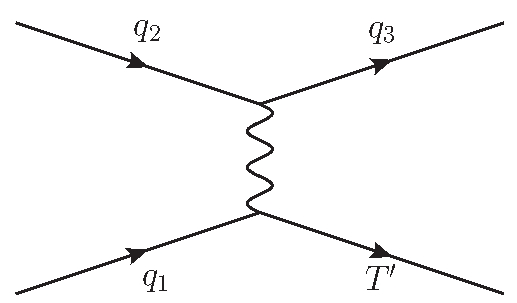
\includegraphics[width=0.3\textwidth]{../figs/Tchannel_T_single.jpg}
    \includegraphics[width=0.35\textwidth]{Hadronization.png}
    \includegraphics[width=0.3\textwidth]{detector_part.png}
  \end{center}
\end{figure}

\end{frame}


\begin{frame}{Parton simulation}
\vspace{-.2cm}

\begin{columns}
\begin{column}{.50\textwidth}
  \begin{block}{}\tiny
    \begin{itemize}
    \item Model proposed to understand collisions of non-fundamental particles.
    \item Valence quarks of a proton are the $u$ and $d$
    \item Sea: $b$, $c$ or $s$ quarks and gluons
    \item Parton distribution function: $f\equiv f(x,Q^{2})$ is the number density of a given quark or gluon as a function of the resolution scale $Q^{2}$ and the fraction of momentum carried by the parton $x$
    \item Simulation done up to a perturbative level: Tree-level or Leading order (LO), one loop or Next-to-Leading-Order (NLO), two loops or Next-to-Next-to-Leading-Order (NNLO), ...
    \end{itemize}
  \end{block}
\vspace{-.3cm}
\begin{block}{}\tiny
\textbf{Tool}: MadGraph $\to$ Matrix-element generator for event generation, calculation of LO cross sections and particle widths. This tool is specially interesting for implementations of BSM models.
\end{block}
\vspace{-.3cm}
\begin{block}{}\tiny
\textbf{Figure}: Martin-Stirling-Thorne-Watt proton PDF for $Q^{2}= 10\, \text{GeV}^{2}$ [left] and $Q^{2}= 10^{4}\, \text{GeV}^{2}$ [right]. $x$ is the fraction of momentum carried by the parton and $f(x,Q^{2})$ the PDF function.
\end{block}
\vspace{-.3cm}
\begin{block}{}\tiny
\textbf{Equation}: $f_{i,j}$ corresponds to the PDF's of the initial partons, $\mathcal{M}_{ij\rightarrow lm}$ is the matrix element of the process
\end{block}
\end{column}

\begin{column}{.50\textwidth}
\begin{figure}[!Hhtbp]
  \begin{center}
    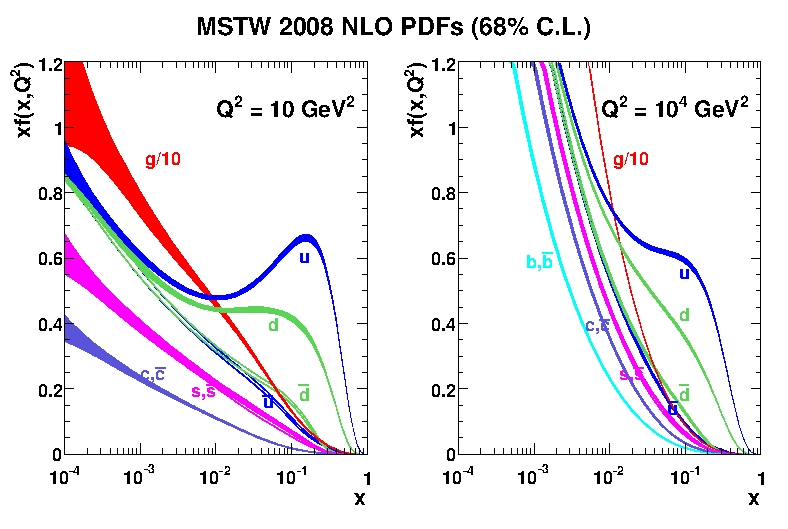
\includegraphics[width=1.0\textwidth]{../figs/mstw2008nlo68cl_allpdfs.jpg}
    %\caption{Martin-Stirling-Thorne-Watt proton PDF for $Q^{2}= 10\, \text{GeV}^{2}$ [left] and $Q^{2}= 10^{4}\, \text{GeV}^{2}$ [right]. $x$ is the fraction of momentum carried by the parton and $f(x,Q^{2})$ the PDF function.}
    %\label{fig:MSTW}
  \end{center}
\end{figure}
\vspace{-.2cm}
{\tiny
\begin{eqnarray}
  %\label{eq:DiffXS}
d\sigma_{ij\rightarrow lm} & = & \left( \int_{0}^{1}\int_{0}^{1}f_{i}(x_{i},Q^{2})f_{j}(x_{j},Q^{2})dx_{i}dx_{j} \right) \nonumber \\
  & \times & \frac{d^{3}p_{l}}{(2\pi)^{2}2E_{l}}\frac{d^{3}p_{m}}{(2\pi)^{2}2E_{m}} \nonumber \\
  & \times & \delta^{4}\left( p_{i}+p_{j}-p_{l}-p_{m} \right) \nonumber \\
  & \times & |\mathcal{M}_{ij\rightarrow lm}|^{2} \nonumber                                     
\end{eqnarray}
}%

\end{column}

\end{columns}
\end{frame}


\begin{frame}{Hadron and Detector simulation}
\vspace{-.2cm}

\begin{columns}
\begin{column}{.50\textwidth}
  \begin{block}{Hadron simulation}\scriptsize
    \begin{itemize}
    \item Quarks produced from hard interaction $\to$ not seen freely due to strong interaction.
    \item Two processes simulations:
      \begin{itemize}\scriptsize
      \item Showering: radiation from initial or final states.
      \item Hadronization: formation of hadrons from final state quarks and gluons.
      \end{itemize}
    \item Hadronization simulation generates the ``soft'' part of the event. Parton simulation generates the hard (interaction) part.
    \end{itemize}
  \end{block}
\vspace{-.3cm}
\begin{block}{}\tiny
\textbf{Tool}: Pythia $\to$ it could take the events produced by a matrix-element generator. If it hadronizes partonic level events, a special procedure (merging) for the interface between the two generations must be done to assure ``physical'' simulations. If not, it generates directly the hadrons from the hard interaction.
\end{block}
\end{column}

\begin{column}{.50\textwidth}
  \begin{block}{Detector simulation}\scriptsize
    \begin{itemize}
    \item Simulation of the detector response to particles simulated in the collision (after hadronization).
    \item Detailed simulation of the detector: subdetectors, cells, layers, electronic cards, ...
    \item It is done as close as possible to reality, however some real detector problems. Two possibilities to solve remaining issues:
      \begin{itemize}\scriptsize
      \item Generate run-dependent MC simulations
      \item Apply corrections to generic MC simulations, to get closer to data.
      \end{itemize}
    \end{itemize}
  \end{block}
\vspace{-.3cm}
\begin{block}{}\tiny
\textbf{Tool}: GEANT 4 $\to$ CMS private detector simulation, with all details of the detector. DELPHES $\to$ Tool to simulate a generic detector with the main pieces: tracking system embedded in a magnetic field, calorimeters and muon system.
\end{block}

\end{column}

\end{columns}
\end{frame}


\begin{frame}{Parton simulation}
\vspace{-.2cm}

\begin{columns}
\begin{column}{.50\textwidth}
  \begin{block}{}
    \tiny \centering 
  \end{block}
\end{column}

\begin{column}{.50\textwidth}

\end{column}

\end{columns}
\end{frame}